\section{Introduction}


\subsection{PCM - Phase Change Memory}

\begin{frame}
\frametitle{Why is PCM interesting as main memory replacement?}

\begin{itemize}
\item Non-volatile
\item 2-4 Times denser than DRAM
\item Read speed comparable to DRAM
\item Uses less energy (doing reads)
\end{itemize}

\end{frame}


\begin{frame}
\frametitle{How does PCM work?}

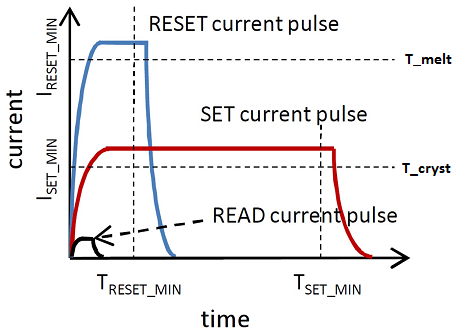
\includegraphics[scale=0.55]{images/set_reset.png}

{\scriptsize
\begin{itemize}
\item \textbf{Reset} pulse (high current$\approx 610^\circ$C) makes the phase change material melt and ``reset'' to a high resistance structure
\item \textbf{Set} pulse (medium/low current$\approx 350^\circ$C) makes the phase change material crystallize, lowering resistance
\item \textbf{Read} Requires almost no current or time at all
\end{itemize}
}
\end{frame}

\begin{frame}
\frametitle{PCM vs. Exiting Memory Technologies}

{\tiny
\begin{tabular}{|l|c|c|c|c|}
\hline
& DRAM & PCM & NAND Flash & HDD \\\hline
Read energy & 0.8 J/GB & 1 J/GB & 1.5 J/GB & 65 J/GB \\
Write energy & 1.2 J/GB & 6 J/GB & 17.5 J/GB & 65 J/GB \\
Idle Power & $_{\tilde{}}\,100$ mW/GB & $_{\tilde{}}\,1$ mW/GB & $_{\tilde{}}\,1-10$ mW/GB & $_{\tilde{}}\,10$ W/GB \\\hline
Endurance & $\infty$ & $10^6-10^8$ & $10^4-10^5$ & $\infty$ \\\hline
Page size & 64B & 64B & 4kB & 512B \\
Page read latency & 20-50ns & $_{\tilde{}}\,50ns$ & $_{\tilde{}}\,25\mu s$ & $_{\tilde{}}\,5 ms$ \\
Page Write latency & 20-50ns & $_{\tilde{}}\,1\mu s$ & $_{\tilde{}}\,500\mu s$ & $_{\tilde{}}\,5 ms$ \\
Write bandwidth & $_{\tilde{}}\,GB/s$ per die & 50-100 MB/s per die & 5-40 MB/s per die & $_{\tilde{}}\,200$ MB/s per drive \\
Erase latency & N/A & N/A & $_{\tilde{}}\,2ms$ & N/A \\\hline
Density & 1X & 2-4X & 4X & N/A \\\hline
\end{tabular}
}
\end{frame}



\begin{frame}
\frametitle{Memory Organization Models}

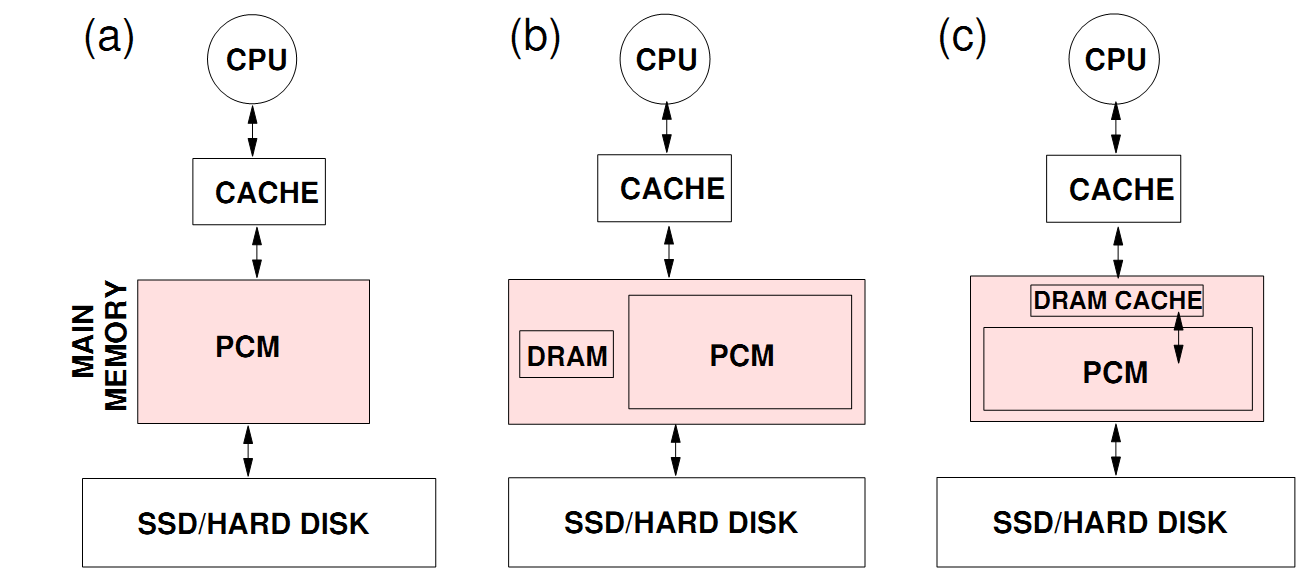
\includegraphics[scale=0.3]{images/memoryorganization.png}
\end{frame}


\subsection{Prior Work}

\begin{frame}
\frametitle{Prior Work}

\begin{itemize}
\item \textbf{CM Architecture}
\item \textbf{PCM-Based File Systems}
\item \textbf{Battery-Backed DRAM (BBDRAM)}
\item \textbf{Main Memory Database Systems and Cache-Friendly Algorithms}
\end{itemize}


\end{frame}




\subsection{Problem}

\begin{frame}
\frametitle{Adapting Core Database algorithms for PCM}

\textbf{How should database systems be modified to best take advantage of the emerging trend towards PCM}

\end{frame}

\begin{frame}
\frametitle{Motivation - Research Interest Growing}

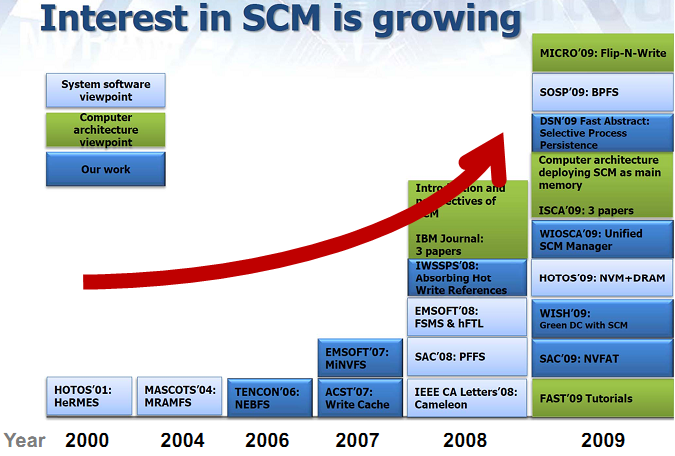
\includegraphics[scale=0.6]{images/growinginterest.png}

\end{frame}




\subsection{Contribution}

\begin{frame}
\frametitle{Contribution}

\begin{itemize}
\item Describe the Unique Characteristics of PCM and it's proposed use as the primary main memory.
\item Present analysis metrics for PCM endurance, energy, and latency.
\item Experimentally show that the proposed algorithms outperform prior versions in terms of time, energy and endurance.
\end{itemize}

\end{frame}